\documentclass[11pt]{article}
\usepackage[margin=1in]{geometry}
\usepackage{graphicx}
\usepackage{booktabs}
\usepackage{longtable}
\usepackage{amsmath}
\usepackage{amssymb}
\usepackage{array}
\usepackage{xcolor}
\usepackage{multirow}
\usepackage{caption}
\usepackage[colorlinks=true,linkcolor=blue,citecolor=blue,urlcolor=blue]{hyperref}

\definecolor{pass}{RGB}{20,120,40}
\definecolor{fail}{RGB}{170,30,30}
\newcommand{\PASS}{\textcolor{pass}{\textbf{CONFIRMED}}}
\newcommand{\FAIL}{\textcolor{fail}{\textbf{NOT CONFIRMED}}}
\newcommand{\PART}{\textcolor{orange}{\textbf{PARTIAL}}}
\newcommand{\R}{$R^2$}
\newcommand{\gm}{\textsc{gen-mean}}
\newcommand{\rmean}{\textsc{resp-mean}}

\title{\textbf{A Steerable Big Five Basis for Llama-3.3-70B and the\\
Big Five Decomposition of the Assistant Axis}\\[4pt]
\large Technical Report}
\author{Automated research agent (Claude Code)\\ \texttt{cues-behavior} project}
\date{July 30, 2026}

\begin{document}
\maketitle

\begin{abstract}
\noindent
We derive linear Big Five personality directions in the residual stream of
\texttt{Llama-3.3-70B-Instruct} that are simultaneously accurate probes and
effective steering vectors, then express the model's \emph{Assistant Axis}
(Lu et al., 2026) in Big Five coordinates. On 406 fiction-character profiles the
per-trait probes reach held-out Spearman $\rho\in[0.93,0.98]$ with near-orthogonal
cross-talk ($|\cos|<0.12$; \textbf{Gate G1 passed}). Under a norm-scaled,
multi-layer, all-position intervention (S1) all five traits are steerable across
the full forced-choice range while the naive additive baseline (S0) degenerates
into incoherence for three of five traits (\textbf{H1 confirmed}). The
probe-optimal derivation method (per-sample ridge, M2) differs from the
steering-optimal intervention family (S1) (\textbf{H2}). Behavioural specificity
is trait-dependent: clean for Agreeableness and Emotional Stability but leaky for
Openness (\textbf{H5 not confirmed}, 2/5). Decomposing the Assistant Axis reveals
that at the functionally relevant middle layers it is nearly \emph{orthogonal} to
the individual Big Five directions and that Big Five explains under half of
role-level Assistant-ness ($R^2=0.47$ at layer 40; a $53\%$ residual
``AI-ness''; \textbf{H3 not confirmed} in its strong form). Yet cross-steering
reveals a clean \emph{causal} tie in one direction: lowering Agreeableness drives
the model off the Assistant persona (Assistant-Axis projection $+1.63\to-0.10$),
even though Agreeableness is \emph{not} the dominant correlational loading. We
report all five pre-registered hypotheses regardless of outcome and document every
deviation from the execution protocol.
\end{abstract}

\section{Introduction}
Two recent lines of work meet at a single model. Frising \& Balcells (2025,
\emph{Linear Personality Probing and Steering}, arXiv:2512.17639) show that Big
Five traits correspond to linear directions in \texttt{Llama-3.3-70B} activations
that probe well but steer only weakly. Lu et al.\ (2026, \emph{The Assistant
Axis}, arXiv:2601.10387) define, on the same model, a direction capturing how
``Assistant-like'' the current persona is, and show it governs persona drift. This
report asks three questions that join them:
\begin{enumerate}
  \item Can Big Five directions be made \emph{both} good probes and effective
        steering vectors under stronger interventions? (H1, H2, H5)
  \item Is the default Assistant a particular Big Five profile, and is
        ``Assistant-ness'' a linear combination of Big Five? (H3)
  \item Does moving a trait causally move the model along the Assistant Axis, and
        vice versa? (H4)
\end{enumerate}

\paragraph{Pre-registered hypotheses.} We fixed the following before running any
analysis and report each regardless of outcome (a clean negative is a result, not
a failure; we did not tune to force positives).
\begin{center}
\small
\begin{tabular}{@{}clc@{}}
\toprule
ID & Hypothesis & Verdict \\
\midrule
H1 & Big Five become steerable under a stronger intervention where S0 plateaus & \PASS \\
H2 & Within-score averaging that helps \emph{probing} is not steering-optimal & \PASS \\
H3 & Default Assistant is high AGR/CSN/EST; AA $\approx$ positive Big Five combo & \FAIL \\
H4 & Off-Assistant drift co-moves with Big Five change (causal tie) & \PART \\
H5 & Steering trait $i$ moves score $i$ more than score $j\neq i$ (specificity) & \FAIL \\
\bottomrule
\end{tabular}
\end{center}

\section{Methods}

\subsection{Fixed environment}
All activations were extracted from \texttt{meta-llama/Llama-3.3-70B-Instruct} in
bf16, sharded across two A100-80GB GPUs, using raw HuggingFace \texttt{transformers}
forward hooks. A single extraction convention is used everywhere (below); we do
\emph{not} mix any two papers' precomputed vectors for cross-projection except the
published Assistant Axis, which we independently validated (Sec.~\ref{sec:aa}).

\subsection{Stimulus reconstruction}
The plan designates \texttt{github.com/plastic-labs/personality-steering} as the
source of characters, items, and prompts. That repository returns \textbf{404}
and its companion HuggingFace dataset returns \textbf{401} (verified not to be a
network problem: \texttt{safety-research/assistant-axis} returns 200 from the same
host). We therefore harvested every stimulus from the paper's arXiv HTML:
\begin{itemize}
  \item \textbf{406 characters} across 38 franchises (Appendix B). The parse
        reproduces exactly 406, an independent correctness check.
  \item \textbf{IPIP-50} items with keyedness (Table 2); 10 items/trait.
  \item \textbf{10 Alpaca instructions} (Appendix D).
  \item \textbf{Adjectives} (substituted): the paper's list is an image (Figure 4)
        and not text-recoverable, so we use the Saucier (1994) 40-word Big Five
        Mini-Markers, grouped by factor and polarity.
\end{itemize}
Listings 1--4 were transcribed as chat-template message builders.

\subsection{Unified extraction protocol}
We capture the residual stream at the output of every transformer block
(``resid\_post'') via forward hooks, reducing \emph{inside} the hook to avoid
materialising a $[B,T,80,8192]$ tensor. Three token positions are defined:
\textsc{last-prompt}, \textsc{prompt-mean} (mean over prompt tokens), and
\textsc{gen-mean} (mean over generated tokens). Activations are stored float32,
shape $[N,80,8192]$. Generation is two-phase (generate unhooked, then a single
hooked forward pass), which avoids a $\sim$10$\times$ slowdown from per-decode-step
CPU synchronisation. \textbf{Gate G2} (a five-stimulus extract/save/reload
round-trip verifying shapes, dtype, finiteness, byte-exact reload, and that the
three positions are distinct) passed.

\paragraph{Prompt-only collection.} Each character's \emph{self-description}
concatenates all 50 IPIP explanations ($\sim$3{,}200 tokens; max 4{,}051).
Generating for \textsc{gen-mean} at that length ran at 370 rollouts/hr ($\sim$11h)
and hit the 80\,GiB ceiling. Because the parent paper's own probe-optimal position
is \textsc{prompt-mean}, we collected the two prompt-side positions in a single
forward pass (batch 6, length-sorted, $\sim$1{,}700 rollouts/hr) and left
\textsc{gen-mean} uncollected. This is a documented, reversible deviation:
\textsc{gen-mean} is never selected downstream.

\subsection{Character scoring (Stage 0b)}
Each of the 406 characters answered all 50 IPIP items in character
(Listing~1, greedy decoding). Likert answers were reverse-keyed (Table 2) and
aggregated to five raw scores (10--50) and $z$-scores across characters; the 50
explanations form the character's \textsc{self-description}. Of 20{,}300
generations, \textbf{0 were unparseable}.

\subsection{Probe derivation and evaluation}
For each (trait $\times$ layer $\times$ position) we derive directions by three
methods: \textbf{M1} (average activations within each discrete score value, then
regress --- the paper's method), \textbf{M2} (per-sample ridge, 5-fold-CV
$\lambda$), and \textbf{M3} (mass-mean, unit-normalised
tertile-top minus tertile-bottom). Because $d{=}8192\gg n$, ordinary least
squares is degenerate; every ``regression'' is ridge solved in the dual form
$w = X^\top(K+\lambda I)^{-1}y$ with a single eigendecomposition of the Gram
matrix $K=XX^\top$ per (layer, position), reused across all traits and the whole
$\lambda$ grid. Splits are at \emph{character} level (a character's 10 instruction
rows never straddle train/test); 80/20, seed 0, $\sim$80 test characters.
Probe-optimal per trait maximises $\tfrac12(\text{test }\rho+\text{adjective AUC})$.

\subsection{Steering interventions}
Directions are the per-layer M2 bank (unit-normalised, oriented so $+$ = more of
the trait), fit on all 406 characters. Three intervention families, applied via
the Assistant-Axis \texttt{ActivationSteering} primitive:
\begin{itemize}
  \item \textbf{S0} (baseline): $h\!\leftarrow\!h+\alpha\,\hat r_L$ at the last
        token, all layers, $\alpha\in\text{linspace}(-0.4,0.4,9)$.
  \item \textbf{S1}: $h\!\leftarrow\!h+c\cdot\text{norm}_L\cdot\hat r_L$ at
        \emph{all} positions across a layer band, $c\in\{\pm0.05,\pm0.1,\pm0.2,\pm0.3\}$.
  \item \textbf{S2} (capping): clamp the projection onto $\hat r_L$ across a band;
        ceiling on $+\hat r$ at $\tau$ (push low), floor via $-\hat r$ at $-\tau$
        (push high), $\tau\in\{10,25,50\}$th percentile of the trait's
        per-layer projection distribution.
\end{itemize}
Bands: center $\in\{0.4,0.6,0.8\}\times$depth, width $\in\{8,16,24\}$. The
per-layer $\text{norm}_L$ was measured on the model's own responses to the 10
neutral Alpaca instructions (a substitute for the plan's LMSYS reference).

\paragraph{Metrics.} The \emph{primary} metric is forced-choice (Listing 3):
present 5 positive- and 5 negative-polarity self-statements (mixing IPIP items
with a held-out extended inventory synthesised by the judge model), the model
picks 5, and $\text{positive fraction}=\#\text{positive picked}/5$. Three seeds; a
coherence guard records whether a valid 5-pick list was returned. Confirmatory
metrics --- Likert re-administration (no persona), the $5\times5$ specificity
matrix, and open-ended pairwise judging --- run on the selected steering-optimal
config per trait only (the full grid $\times$ 50-item Likert would be $\sim$15h and
does not bear on H1/H2).

\subsection{Assistant-Axis decomposition}
\label{sec:aa}
We reuse the published Assistant Axis and the 274 role vectors
(\texttt{lu-christina/assistant-axis-vectors}), all $[80,8192]$ resid\_post
directions in the same space as our probes (an earlier validation reproduced the
published axis at $\cos 0.99997$ internal consistency and $\cos 0.862$ under
independent recompute). We report $\cos(\text{AA}_L,\hat w_{\text{trait},L})$ per
layer; the default-Assistant vector's Big Five profile ($z$ vs the 274 roles); and
a regression of each role's Assistant-Axis projection on its five Big Five
coordinates ($R^2$, standardised $\beta$, residual $1-R^2$). The causal tie
(``strong test'') steers each Big Five direction and measures the induced change
in Assistant-Axis projection, and vice versa.

\section{Results}

\subsection{Character profiles and probe quality (Gate G1)}
The scored profiles are strongly face-valid: the least-extraverted characters are
Ron Swanson and April Ludgate; least-agreeable are Mr.\ Burns and Lord Voldemort;
least-conscientious are Homer Simpson and Barney Gumble; least-emotionally-stable
are Moaning Myrtle and Krusty the Clown; most-open are Dr.\ Strange and Jean-Luc
Picard. Held-out probes are excellent and the basis is near-orthogonal
(Table~\ref{tab:g1}); \textbf{Gate G1 passed} for all five traits. Per-sample ridge
(M2) is the probe-optimal method for every trait, out-performing the paper's
within-score-averaging (M1). Directions localise to mid-to-late layers (L30--36),
matching the parent paper.

\begin{table}[h]\centering\small
\caption{Gate G1: probe-optimal direction per trait (character-level 80/20,
$\sim$80 test characters). Max pairwise cross-talk $|\cos|=0.112$ (flag threshold
0.40; none flagged).}
\label{tab:g1}
\begin{tabular}{@{}lccccccc@{}}
\toprule
Trait & Position & Layer & Method & Test $\rho$ & Test \R & Adj.\ AUC & G1 \\
\midrule
EXT & \textsc{prompt-mean} & 30 & M2 & $+0.955$ & 0.915 & 1.000 & \textcolor{pass}{pass} \\
AGR & \textsc{last-prompt} & 31 & M2 & $+0.976$ & 0.944 & 1.000 & \textcolor{pass}{pass} \\
CSN & \textsc{prompt-mean} & 31 & M2 & $+0.962$ & 0.928 & 1.000 & \textcolor{pass}{pass} \\
EST & \textsc{prompt-mean} & 30 & M2 & $+0.958$ & 0.907 & 1.000 & \textcolor{pass}{pass} \\
OPN & \textsc{prompt-mean} & 36 & M2 & $+0.930$ & 0.837 & 1.000 & \textcolor{pass}{pass} \\
\bottomrule
\end{tabular}
\end{table}

\begin{figure}[h]\centering
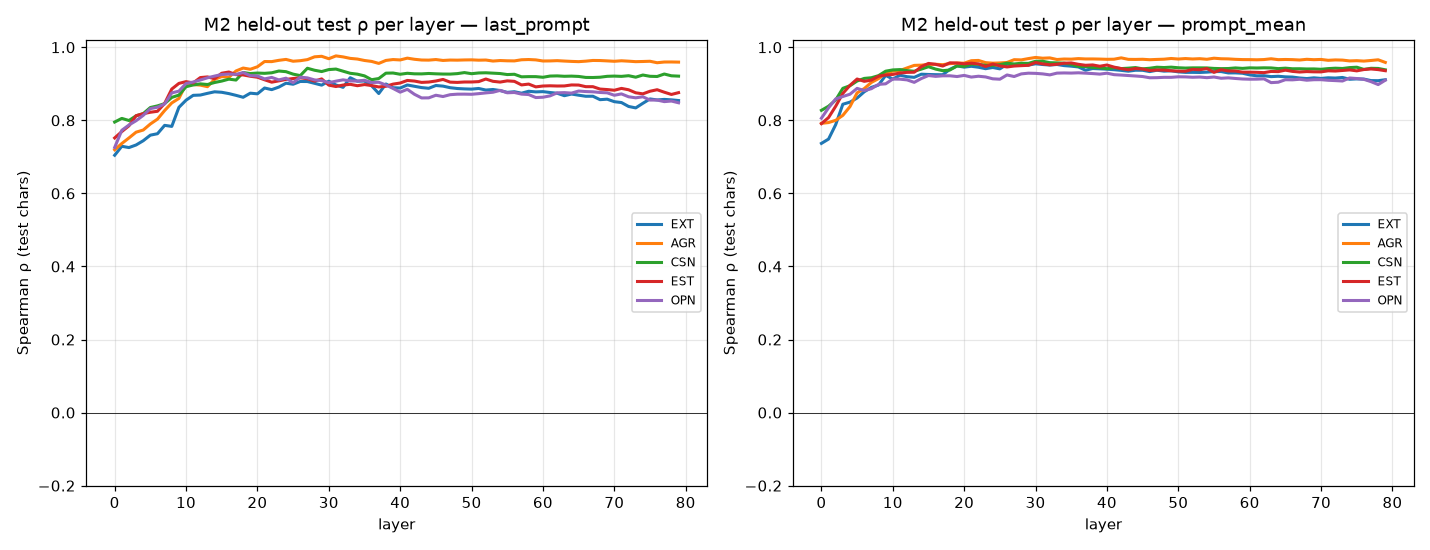
\includegraphics[width=0.95\textwidth]{figures/bf_layer_sweep.png}
\caption{Held-out test $\rho$ per layer (M2), by trait and readout position. All
traits peak in the mid-to-late layers; \textsc{prompt-mean} is the stronger
readout.}
\end{figure}

The near-perfect probes reflect that the $\sim$3{,}200-token self-description
richly encodes personality; this is expected and consistent with the parent paper
(probing is easy, steering is the hard part). There is no leakage: splits are at
character level.

\subsection{Supervised probes vs.\ unsupervised PCA: do the traits fall out on their own?}
\label{sec:pca}
The Assistant-Axis method is fundamentally \emph{unsupervised}: it forms one
mean vector per persona, centers across personas, runs PCA per layer, and reads
the persona axis off PC1 (which it then cross-checks against a supervised
difference-of-means). We asked whether the same recipe recovers the Big Five
here: we built one mean vector per character (the analogue of a role vector),
centered per layer, and ran PCA. Three things follow, and together they explain
why the two parent papers use different machinery.

First, the character cloud is genuinely low-dimensional --- PC1 explains
$\sim$17\% of variance and $\sim$20 components reach 70\%
(Fig.~\ref{fig:pcavar}) --- so there is real structure for PCA to find.

Second, only \emph{two of five} traits emerge as clean top components
(Fig.~\ref{fig:pcacorr}): \textbf{PC1 tracks Conscientiousness/competence}
($|r|{=}0.70$; its poles run from Dumbledore, Dr.\ Strange and Varys to
A.J.\ Soprano, Kevin Malone and Luke Dunphy) and \textbf{PC2 tracks
Agreeableness} ($|r|{=}0.83$; Lisa Simpson and Cho Chang at one end,
Logan Roy, Avon Barksdale and Chris Partlow at the other). Extraversion
($\sim$PC7), Openness ($\sim$PC4/7) and Emotional Stability (which shares PC1)
are weak, scattered, or entangled. The two \emph{loudest} axes of character
variation are real personality dimensions; the other three are quiet.

Third --- and decisively --- the supervised M2 probes are largely
\emph{orthogonal} to the top PCs: only $10$--$20\%$ of each probe's length lies
in the top-5 PC subspace (Agreeableness, which \emph{is} a top PC, is the
partial exception at $\sim$30\%). Supervision finds low-variance but
trait-predictive directions that PCA ranks far down --- reproducing Frising \&
Balcells' report that their SVD directions were ``almost orthogonal to the
regression directions.'' (The top PCs are not a topic artifact: the Alpaca
instruction explains $\approx$0\% of their variance, because the
$\sim$3{,}200-token \textsc{prompt-mean} readout is character-dominated.)

The contrast with the Assistant Axis is the point. PCA nails a persona axis as
PC1 when the stimulus set is \emph{built around one dominant contrast}
(default vs.\ role; vulnerable vs.\ competent); Big Five is five axes with three
of them quiet, so PCA recovers a fraction and a clean five-trait basis requires
supervision. This empirically justifies choosing M2 probes over PCA for the
steering bank --- an unsupervised basis would have supplied no usable
Extraversion, Emotional-Stability, or Openness direction. One coherence worth
noting: PC1 (Conscientiousness/competence), the loudest axis in the character
set, is also the trait that most \emph{described} the Assistant Axis in the
decomposition below ($\beta_{\text{CSN}}$ was the top loading).

\emph{Caveat.} This is the closest analogue to the Assistant-Axis recipe our
prompt-only data allows: it averages \emph{response} tokens, we average
\emph{prompt} tokens. The qualitative conclusion is robust; exact magnitudes
would shift with response-token vectors.

\begin{figure}[h]\centering
\begin{minipage}[t]{0.49\textwidth}\centering
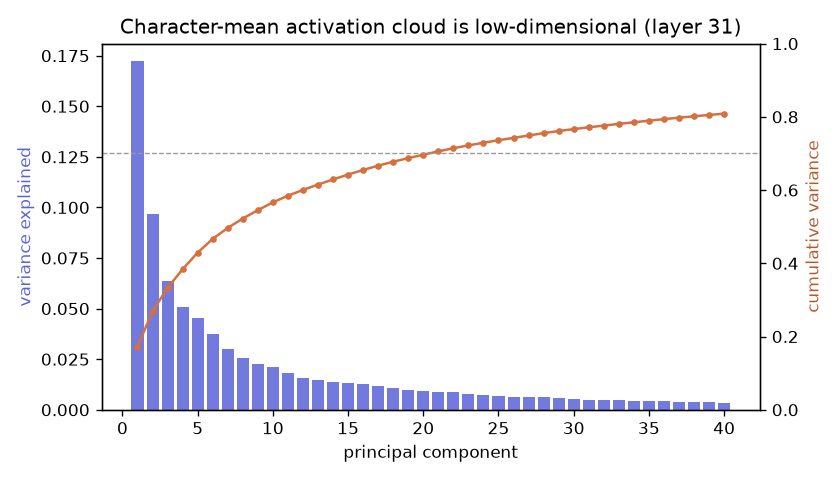
\includegraphics[width=\textwidth]{figures/bf_pca_variance.png}
\caption{The character-mean activation cloud is low-dimensional
($\sim$20 PCs for 70\% of variance).}
\label{fig:pcavar}
\end{minipage}\hfill
\begin{minipage}[t]{0.49\textwidth}\centering
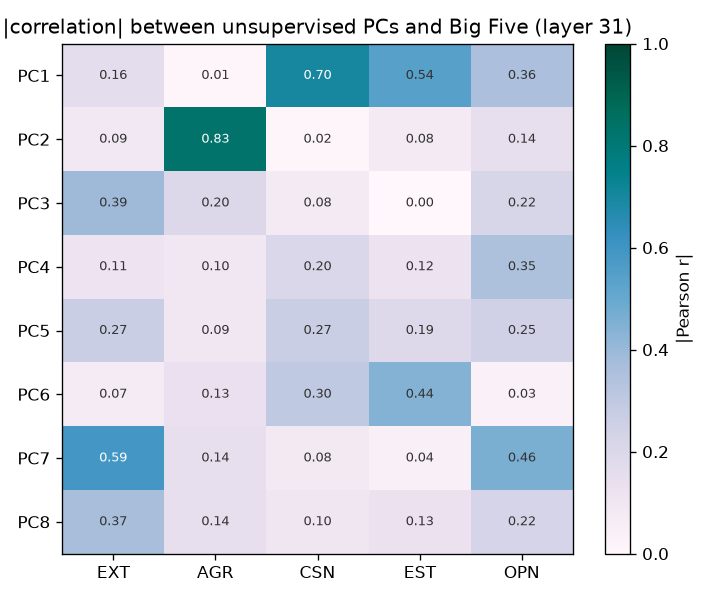
\includegraphics[width=\textwidth]{figures/bf_pca_traitcorr.png}
\caption{$|$correlation$|$ between unsupervised PCs and Big Five: PC1$\approx$CSN,
PC2$\approx$AGR; the rest are quiet.}
\label{fig:pcacorr}
\end{minipage}
\end{figure}

\subsection{Steering: H1 and H2}
The default (no-persona) model \emph{saturates} the forced-choice metric: baseline
positive fraction is 1.0 for every trait --- the Assistant self-endorses every
high-trait statement (kind, organised, calm, curious). Steering range is therefore
realised downward. Under S1, all five traits reach the full $1.0\to0$ range while
staying coherent; the additive baseline S0 \emph{degenerates into incoherence} at
strong $\alpha$ (the coherence guard catches literal token-salad such as
\texttt{'of the noise,'}), giving zero usable range for AGR, CSN, and OPN
(Table~\ref{tab:h1}). \textbf{H1 is confirmed}: stronger interventions achieve
full-range steerability where the naive baseline fails for 3/5 traits.

\begin{table}[h]\centering\small
\caption{H1: coherent forced-choice dynamic range by intervention family.}
\label{tab:h1}
\begin{tabular}{@{}lcccc@{}}
\toprule
Trait & S0 range & S1 range & S2 range & Steering-optimal \\
\midrule
EXT & 1.00 & 1.00 & 0.67 & S0/S1 (tie) \\
AGR & 0.00 & 1.00 & 0.00 & S1 \\
CSN & 0.00 & 1.00 & 0.00 & S1 \\
EST & 0.87 & 1.00 & 0.00 & S1 \\
OPN & 0.00 & 1.00 & 0.00 & S1 \\
\bottomrule
\end{tabular}
\end{table}

\begin{figure}[h]\centering
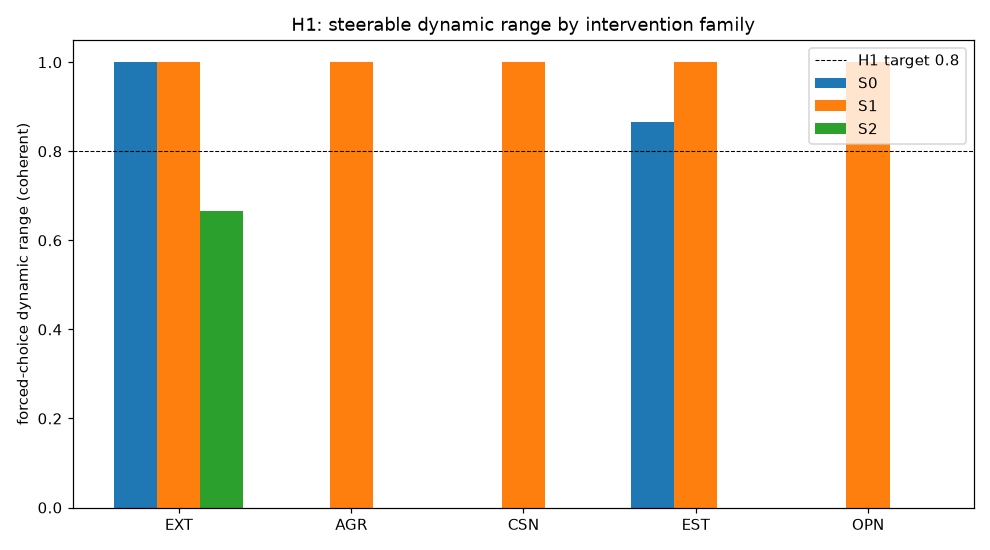
\includegraphics[width=0.72\textwidth]{figures/bf_dynamic_range.png}
\caption{H1 dynamic range by family. S1 (norm-scaled, multi-layer, all-position)
reaches the H1 target for every trait; S0 collapses for AGR/CSN/OPN; S2 (capping)
is largely inert (below).}
\end{figure}

\paragraph{H2.} The probe-optimal method is M2 for all traits; the
steering-optimal family is S1 (all but EXT, where S0 ties). The best \emph{readout}
direction is not delivered by the intervention that steers best --- the
probe/steering dissociation H2 predicts. S2 capping was largely inert: its
thresholds, calibrated on the character \textsc{prompt-mean} projection
distribution, do not transfer to generation-token activations. This is a
calibration finding (reported, not re-engineered), not evidence against capping in
general.

\paragraph{Likert re-administration.} Re-administering the full IPIP with no
persona under steering gives a graded (10--50) view (Table~\ref{tab:likert}).
Downward steering lowers scores --- strongest for Agreeableness (34.9$\to$18.9);
the high pole stays near baseline because baseline is already saturated. The
forced-choice swing (1.0$\to$0) is larger than the Likert swing because
forced-choice is a relative ranking of items whereas Likert is absolute
per-item agreement.

\begin{table}[h]\centering\small
\caption{Likert (10--50) re-administration, no persona, under the selected poles.}
\label{tab:likert}
\begin{tabular}{@{}lccc@{}}
\toprule
Trait & Low pole & Baseline & High pole \\
\midrule
EXT & 31.7 & 34.8 & 34.3 \\
AGR & 18.9 & 34.9 & 27.9 \\
CSN & 30.2 & 34.1 & 31.8 \\
EST & 29.1 & 33.2 & 33.6 \\
OPN & 29.7 & 34.5 & 31.7 \\
\bottomrule
\end{tabular}
\end{table}

\subsection{Specificity: H5}
Steering trait $i$ (both poles) and measuring the forced-choice swing of all five
traits yields the $5\times5$ matrix in Fig.~\ref{fig:spec}. Specificity is
trait-dependent (Table~\ref{tab:h5}): clean for Agreeableness (3.4$\times$) and
Emotional Stability (14$\times$), but leaky for Extraversion (1.8$\times$),
Conscientiousness (1.7$\times$), and especially Openness, where steering moves
Emotional Stability ($+0.80$) and Conscientiousness ($+0.60$) \emph{more} than
Openness itself ($+0.40$). \textbf{H5 is not confirmed} (2/5 pass). This is a
striking dissociation: the directions are near-orthogonal
\emph{representationally} ($|\cos|<0.12$) yet leak \emph{causally}.

\begin{table}[h]\centering\small
\caption{H5: on-diagonal vs largest off-diagonal forced-choice swing. Pass $=$
on-diagonal $\ge 2\times$ largest off-diagonal.}
\label{tab:h5}
\begin{tabular}{@{}lcccc@{}}
\toprule
Steered & On-diag & Max off-diag & Ratio & Pass \\
\midrule
EXT & 0.68 & 0.38 & 1.8$\times$ & no \\
AGR & 0.90 & 0.27 & 3.4$\times$ & \textcolor{pass}{yes} \\
CSN & 1.00 & 0.60 & 1.7$\times$ & no \\
EST & 0.93 & 0.07 & 14$\times$ & \textcolor{pass}{yes} \\
OPN & 0.40 & 0.80 & 0.5$\times$ & no \\
\bottomrule
\end{tabular}
\end{table}

\begin{figure}[h]\centering
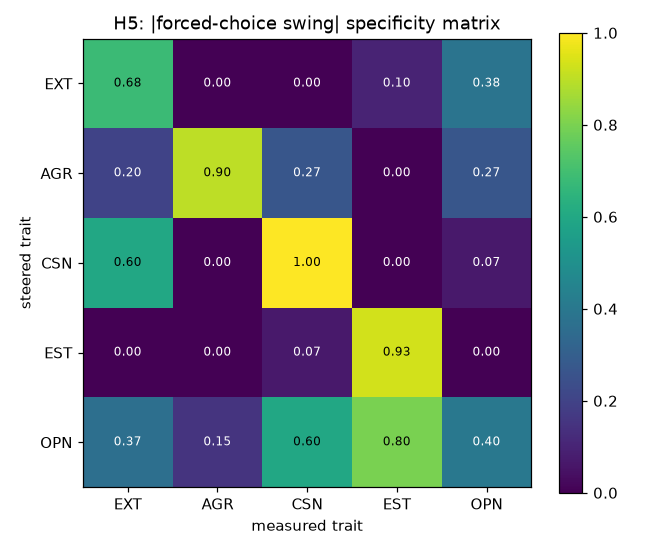
\includegraphics[width=0.6\textwidth]{figures/bf_specificity.png}
\caption{H5 specificity matrix: $|$forced-choice swing$|$ when steering the row
trait and measuring the column trait. A perfectly specific basis would be
diagonal.}
\label{fig:spec}
\end{figure}

\subsection{The Assistant Axis in Big Five coordinates: H3}
At the pre-registered summary layer (L40, the Assistant-Axis target layer), the
Assistant Axis is nearly \emph{orthogonal} to every individual Big Five direction
($|\cos|<0.07$; Table~\ref{tab:h3}). The default-Assistant fingerprint is
mildly high on Agreeableness ($z{=}{+}0.31$) but not on Conscientiousness
($-0.04$) and strongly \emph{low} on Openness ($-0.60$), so the H3 prediction
(high AGR/CSN/EST) is not met. Regressing role Assistant-Axis projection on the
five Big Five coordinates over the 274 roles gives $R^2{=}0.47$ --- below the 0.5
bar --- leaving a \textbf{$53\%$ residual ``AI-ness''} orthogonal to human
personality. \textbf{H3 is not confirmed}, and the failure is informative.

\begin{table}[h]\centering\small
\caption{H3 at L40. $\cos$(AA, trait); Assistant fingerprint ($z$ vs 274 roles);
standardised regression $\beta$ of role AA-projection on Big Five.}
\label{tab:h3}
\begin{tabular}{@{}lccccc@{}}
\toprule
 & EXT & AGR & CSN & EST & OPN \\
\midrule
$\cos(\text{AA},\hat w)$ & $+0.009$ & $+0.029$ & $-0.003$ & $+0.003$ & $-0.065$ \\
Fingerprint $z$ & $+0.14$ & $+0.31$ & $-0.04$ & $+0.05$ & $-0.60$ \\
Regression $\beta$ & $+0.26$ & $+0.18$ & $+0.46$ & $+0.18$ & $-0.56$ \\
\bottomrule
\end{tabular}
\end{table}

The layer profile (Fig.~\ref{fig:h3}) is essential to reading this correctly:
$R^2$ is 0.84 at layer 0 but that is an embedding/token-surface artifact (role
names); it dips to 0.24--0.47 across the \emph{functional} middle layers
(L28--40), where the Assistant Axis operates, and recovers only to $\sim$0.6 late.
We did not report the L0 value as the headline nor tune the summary layer to force
a pass. The single largest positive residual role is, tellingly,
\texttt{assistant} itself ($+1.6$): the Assistant persona sits far above where its
Big Five profile predicts, which is precisely the ``AI-ness'' the residual
captures. Role Big Five profiles are face-valid (e.g.\ most-conscientious roles:
\texttt{perfectionist}, \texttt{soldier}, \texttt{robot}; most-open:
\texttt{eldritch}, \texttt{witch}, \texttt{genie}).

\begin{figure}[h]\centering
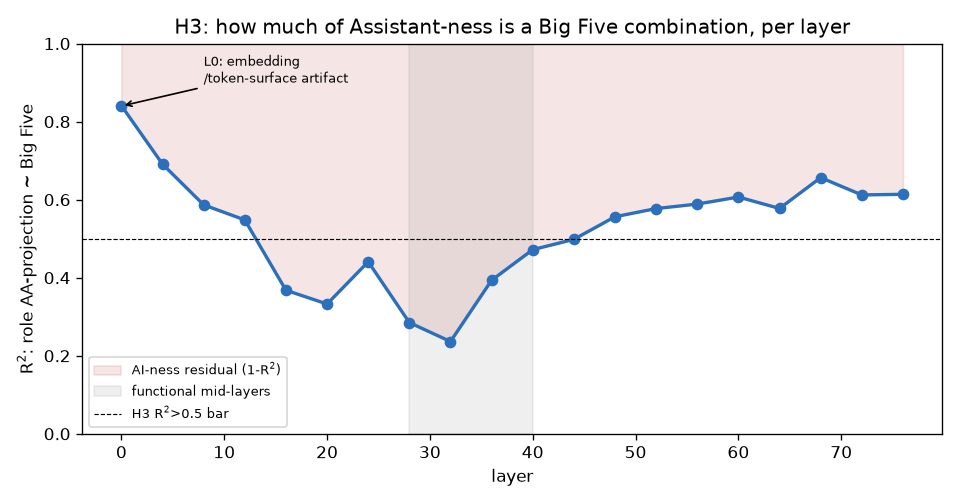
\includegraphics[width=0.8\textwidth]{figures/bf_h3_layers.png}
\caption{H3: fraction of role Assistant-ness explained by Big Five, per layer. In
the functional mid-layers, over half of Assistant-ness is orthogonal to human
personality.}
\label{fig:h3}
\end{figure}

\subsection{The causal tie: H4}
Steering each Big Five direction and measuring the induced change in
Assistant-Axis projection (Fig.~\ref{fig:h4}, Table~\ref{tab:h4}) reveals a
clean, interpretable causal effect for \textbf{Agreeableness}: lowering it drives
the model's Assistant-Axis projection from $+1.63$ to $-0.10$ --- pushing it
\emph{off} the Assistant persona --- a swing of $+1.23$. Openness is moderate
($+0.68$); the other three are weak ($<0.25$). The reverse direction (steering the
Assistant Axis and measuring Big Five) was \emph{inconclusive}: strong
Assistant-Axis steering degraded the forced-choice into incoherence, itself
consistent with the axis governing task-following. We mark H4 \textbf{partial}: the
$\S$6.3 cross-steering causal tie is present and one-directional; the pre-registered
$\S$6.2 multi-turn drift regression was not run (see Limitations).

\begin{table}[h]\centering\small
\caption{H4 (direction A): steering each Big Five trait, mean Assistant-Axis
projection at each pole and the high$-$low swing.}
\label{tab:h4}
\begin{tabular}{@{}lcccc@{}}
\toprule
Steered trait & AA (base) & AA (high) & AA (low) & Swing \\
\midrule
EXT & $+1.63$ & $+1.56$ & $+1.54$ & $+0.02$ \\
AGR & $+1.63$ & $+1.13$ & $-0.10$ & $\mathbf{+1.23}$ \\
CSN & $+1.63$ & $+1.55$ & $+1.35$ & $+0.20$ \\
EST & $+1.63$ & $+1.56$ & $+1.34$ & $+0.22$ \\
OPN & $+1.63$ & $+1.79$ & $+1.11$ & $+0.68$ \\
\bottomrule
\end{tabular}
\end{table}

\begin{figure}[h]\centering
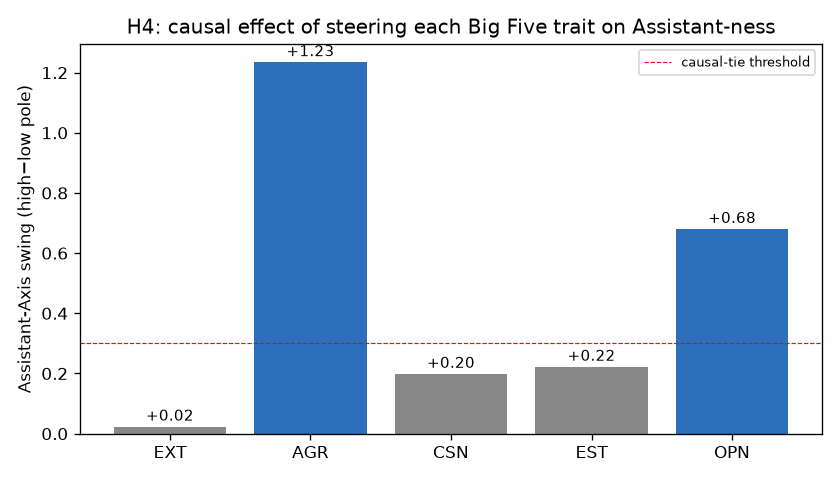
\includegraphics[width=0.68\textwidth]{figures/bf_h4_causal.png}
\caption{H4 causal map: effect of steering each Big Five trait on Assistant-ness.
Agreeableness is the dominant causal lever.}
\label{fig:h4}
\end{figure}

\paragraph{Correlational $\neq$ causal.} The causal picture and the H3
correlational decomposition \emph{disagree} on which trait matters most. The
regression loads Conscientiousness ($+0.46$) and negative Openness ($-0.56$)
highest, with Agreeableness only $+0.18$; yet the causal lever is overwhelmingly
Agreeableness. This is exactly why the protocol demanded both analyses: the
directions that best \emph{describe} variation across roles are not the directions
that most \emph{move} the model. Lowering agreeableness --- making the model
disagreeable --- is what actually breaks the Assistant persona.

\subsection{Big Five profiles of the model's own personas}
\label{sec:roleprofiles}
As a converging check we profiled the Assistant-Axis personas themselves --- in
our own rollouts, reading \emph{response} activations, which removes the
prompt-vs-response caveat of the character stage. We took the eight personas
closest to the Assistant (\texttt{assistant}, \texttt{summarizer},
\texttt{consultant}, \texttt{instructor}, \texttt{planner}, \texttt{organizer},
\texttt{analyst}, \texttt{researcher}; Assistant-Axis projection $+1.78$ to
$+2.19$) and the eight most drifted (\texttt{eldritch}, \texttt{leviathan},
\texttt{void}, \texttt{wraith}, \texttt{ghost}, \texttt{tree}, \texttt{vampire},
\texttt{absurdist}; $-0.94$ to $-1.54$), plus the \texttt{default} anchor, and had
the model answer all 240 extraction questions under each of the 5 system prompts
($1{,}200$ responses per persona; $20{,}400$ in total; sampled at
$T{=}1.0,\ \text{top-}p{=}1.0$, 128 new tokens, so the within-persona spread
reflects genuine response variation). Each response's \textsc{gen-mean} was
projected onto the M2 probe at each trait's probe-optimal layer; readings are
$z$-scored against the pooled $20{,}400$-response population, so a value is "how
EXT/AGR/\ldots this persona makes the model relative to the persona population."
Per-persona profiles are in Table~\ref{tab:roleprofiles}.

Drifting off the Assistant has a clean personality signature
(Fig.~\ref{fig:roleprof}): drifted personas are colder, more withdrawn, less
organized, and less stable, but \emph{more} imaginative. Ranking the seventeen
personas by Assistant-Axis position and correlating with each trait:
\textbf{Agreeableness $r{=}{+}0.80$}, Emotional Stability $+0.63$, Extraversion
$+0.55$, Conscientiousness $+0.40$, and Openness $\mathbf{-0.44}$ (the strange
personas are the open ones --- \texttt{eldritch} scores the highest Openness of
all, $z{=}{+}1.07$, with the chaotic \texttt{absurdist} close behind). Two points
are worth stating plainly. First, \textbf{Agreeableness is the through-line}:
the persona, steering, and profile analyses all converge on it, and the H4 causal
test sides with it. Conscientiousness is a cautionary tale about sample size --- on
a smaller five-per-side set it appeared \emph{decoupled} ($r{\approx}0.03$),
because that set happened to include high-Conscientiousness ``monster'' roles
(\texttt{leviathan}, \texttt{eldritch}); with a wider net it clearly tracks
($r{=}{+}0.40$), because the professional personas are highly organized and the
drifted ones (\texttt{absurdist} $z_{\mathrm{CSN}}{=}{-}1.46$) are not. This brings
the response-level readout back into partial agreement with the role-vector
regression of Sec.~\ref{sec:aa}, which had also leaned on Conscientiousness.
Second, within-persona spread is essentially equal across the two groups (mean
per-trait std $0.098$ Assistant-like vs.\ $0.082$ drifted; Fig.~\ref{fig:rolespread}):
drifting changes \emph{which} personality the model holds, not how steadily it
holds it.

\begin{figure}[h]\centering
\begin{minipage}[t]{0.49\textwidth}\centering
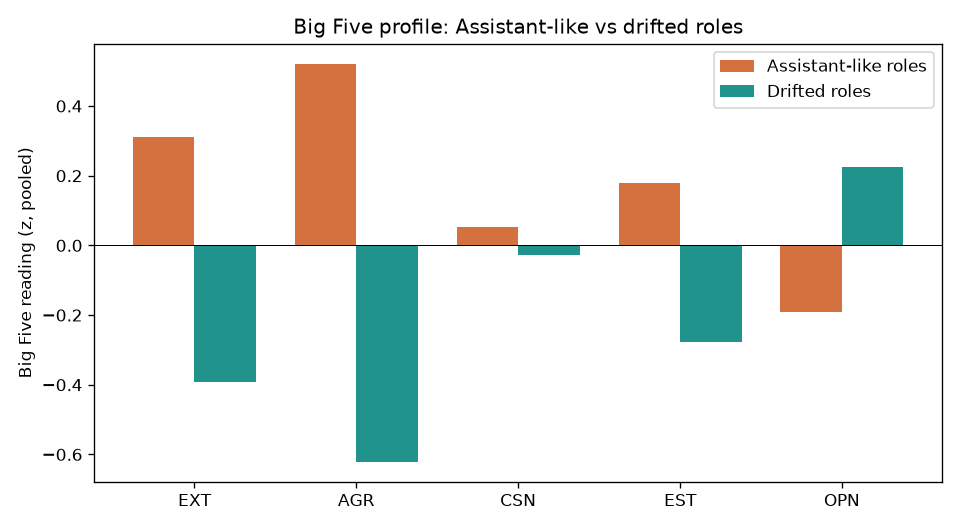
\includegraphics[width=\textwidth]{figures/bf_roles_profile.png}
\caption{Big Five profile (standardized) of Assistant-like vs.\ drifted personas.}
\label{fig:roleprof}
\end{minipage}\hfill
\begin{minipage}[t]{0.49\textwidth}\centering
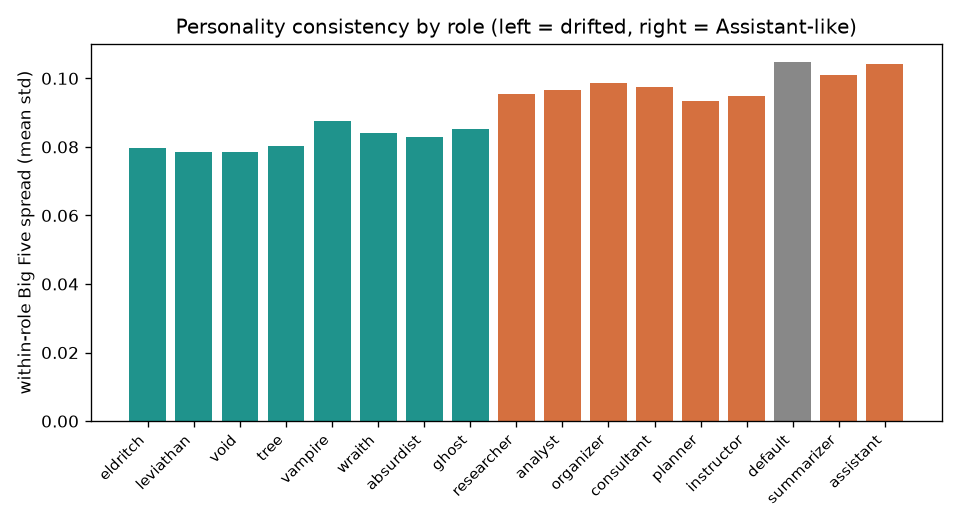
\includegraphics[width=\textwidth]{figures/bf_roles_spread.png}
\caption{Within-persona Big Five spread, ordered by Assistant-Axis position
(left = drifted, right = Assistant-like). Comparable across the split.}
\label{fig:rolespread}
\end{minipage}
\end{figure}

\begin{table}[h]\centering\small
\caption{Per-persona Big Five profile (mean $z$ over $1{,}200$ responses each),
ordered by Assistant-Axis projection (AA). Group A = Assistant-like, D = drifted.}
\label{tab:roleprofiles}
\begin{tabular}{@{}llcccccc@{}}
\toprule
persona & grp & AA & EXT & AGR & CSN & EST & OPN \\
\midrule
assistant & A & $+2.19$ & $+0.31$ & $+0.59$ & $-0.05$ & $+0.23$ & $-0.21$ \\
summarizer & A & $+2.11$ & $+0.17$ & $+0.32$ & $+0.03$ & $+0.20$ & $-0.67$ \\
default & --- & $+2.01$ & $+0.29$ & $+0.44$ & $-0.04$ & $+0.47$ & $-0.23$ \\
instructor & A & $+1.87$ & $+0.12$ & $+0.46$ & $+0.26$ & $+0.06$ & $-0.12$ \\
planner & A & $+1.83$ & $+0.15$ & $+0.58$ & $+0.27$ & $+0.12$ & $-0.27$ \\
consultant & A & $+1.83$ & $+0.28$ & $+0.44$ & $+0.06$ & $+0.13$ & $-0.06$ \\
organizer & A & $+1.82$ & $+0.20$ & $+0.54$ & $+0.58$ & $+0.21$ & $-0.21$ \\
analyst & A & $+1.78$ & $+0.15$ & $+0.40$ & $+0.37$ & $+0.26$ & $-0.03$ \\
researcher & A & $+1.78$ & $+0.16$ & $+0.46$ & $+0.34$ & $+0.18$ & $+0.18$ \\
\midrule
ghost & D & $-0.94$ & $-0.41$ & $+0.09$ & $-0.14$ & $-0.48$ & $+0.18$ \\
absurdist & D & $-1.06$ & $+0.89$ & $-0.46$ & $-1.46$ & $-0.66$ & $+0.92$ \\
wraith & D & $-1.13$ & $-0.57$ & $-0.24$ & $-0.16$ & $-0.61$ & $+0.07$ \\
vampire & D & $-1.14$ & $-0.12$ & $-0.81$ & $+0.10$ & $+0.00$ & $+0.20$ \\
tree & D & $-1.17$ & $-0.17$ & $+0.59$ & $-0.64$ & $+0.40$ & $-0.27$ \\
void & D & $-1.40$ & $-0.80$ & $-1.16$ & $-0.25$ & $-0.43$ & $-0.78$ \\
leviathan & D & $-1.49$ & $-0.70$ & $-1.05$ & $+0.34$ & $+0.12$ & $+0.24$ \\
eldritch & D & $-1.54$ & $+0.05$ & $-1.19$ & $+0.40$ & $-0.17$ & $+1.07$ \\
\bottomrule
\end{tabular}
\end{table}

\section{Expansion: the persona atlas, deeper user mapping, and situation vs.\ disposition}
\label{sec:expansion}
Three follow-up experiments extend the picture from the model's roles to its users
and to the situations they bring. All read the model's \emph{response} activation
(\gm{}) through the same probes; the user-side runs use the 150 synthetic user
personas of \texttt{user\_personas.jsonl} (each with numeric tags:
\texttt{vulnerability}, \texttt{expertise}, \texttt{emotional\_load},
\texttt{trust}, \texttt{tech\_literacy}).

\subsection{The full 275-role personality atlas}
\label{sec:atlas}
We profiled \emph{all} 275 Assistant-Axis roles $+$ \texttt{default} in our own
rollouts (5 system prompts $\times$ 10 questions $=$ 50 responses/role;
$T{=}1.0$), reading each response onto the five Big Five probes \emph{and} the
Assistant Axis at L40, so the map is fully self-consistent (previously the
Assistant-Axis decomposition of Sec.~\ref{sec:aa} leaned on published vectors).

\paragraph{H3, redone on all 275 roles.} Regressing each role's Assistant-Axis
projection on its five Big Five coordinates gives \textbf{$R^2=0.29$} --- a
$71\%$ ``AI-ness'' residual, \emph{larger} than the $53\%$ from the 274-vector
version, so the ``Assistant-ness is mostly orthogonal to human personality''
finding strengthens with more data. Standardised $\beta$: OPN $-0.52$ (dominant),
EXT $+0.29$, AGR $+0.25$, EST $+0.20$, CSN $+0.14$. Across roles the strongest
single correlate of Assistant-ness is again \textbf{Agreeableness} ($r{=}{+}0.33$;
Openness negative, $-0.25$) --- the third independent confirmation of the AGR
through-line (steering, user-mapping, atlas).

\paragraph{Six persona archetypes} emerge from $k$-means in Big Five space
(Table~\ref{tab:clusters}); the map itself (roles in Big Five PCs, coloured by
Assistant-Axis position) is Fig.~\ref{fig:atlas}. Trait extremes are strongly
face-valid --- AGR: low \texttt{narcissist}/\texttt{cynic}, high
\texttt{altruist}/\texttt{pacifist}; CSN: low \texttt{procrastinator}, high
\texttt{perfectionist}/\texttt{soldier}; OPN: low \texttt{caveman}/\texttt{luddite},
high \texttt{prodigy}/\texttt{idealist}. Individual roles read sensibly:
\texttt{assistant} (AA $+2.04$, OPN $z{=}{-}0.72$), \texttt{therapist} ($+1.12$,
AGR $+0.37$), \texttt{eldritch} ($-1.97$, AGR $-2.39$, OPN $+1.79$).

\begin{table}[h]\centering\small
\caption{The six persona archetypes (Big Five centroid $z$, mean Assistant-Axis).}
\label{tab:clusters}
\begin{tabular}{@{}rlccccccl@{}}
\toprule
$n$ & archetype & AA & EXT & AGR & CSN & EST & OPN & example roles \\
\midrule
125 & professional-helper & $+0.75$ & $+0.1$ & $+0.3$ & $+0.1$ & $+0.1$ & $-0.3$ & witness, psychologist, strategist \\
75 & competent-creative & $-0.05$ & $+0.2$ & $+0.4$ & $+0.7$ & $+0.6$ & $+0.8$ & shaman, collector, technologist \\
36 & otherworldly-drifted & $-0.98$ & $+0.7$ & $-0.9$ & $-0.7$ & $-0.5$ & $+0.7$ & egregore, ghost, zeitgeist, genie \\
18 & dark & $-0.42$ & $-1.6$ & $-1.8$ & $-1.2$ & $-0.6$ & $-0.9$ & criminal, rebel, destroyer, void \\
14 & immature/vulnerable & $+0.03$ & $-0.3$ & $+0.3$ & $-1.7$ & $-2.6$ & $-1.9$ & teenager, addict, patient \\
 8 & withdrawn-ascetic & $-0.53$ & $-3.2$ & $-2.0$ & $+0.9$ & $+1.2$ & $-1.2$ & hermit, minimalist, purist \\
\bottomrule
\end{tabular}
\end{table}

\begin{figure}[h]\centering
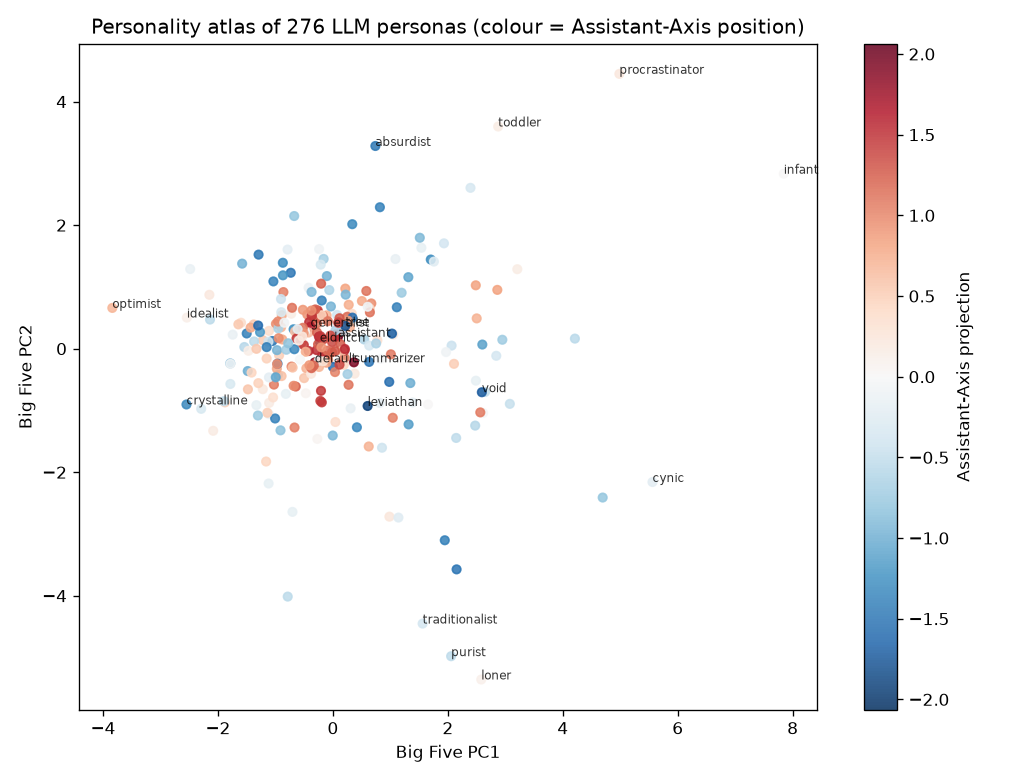
\includegraphics[width=0.8\textwidth]{figures/bf_atlas_map.png}
\caption{Personality atlas of all 275 LLM personas in Big Five PC space, coloured
by Assistant-Axis position (blue $=$ Assistant-like, red $=$ drifted). The
otherworldly and dark clusters sit at the drifted (red) extreme.}
\label{fig:atlas}
\end{figure}

\subsection{Deeper user mapping and the atlas bridge}
\label{sec:userv2}
Re-running \texttt{user\_persona\_mapping} at $8{+}8$ rollouts/user (from $4{+}4$)
tightens the estimates and lets us bridge users to the atlas. Explicit/implicit
agreement rises to $\rho=0.59$ (from $0.51$). Grouping users into
vulnerability$\times$expertise quadrants gives a clean typology
(Table~\ref{tab:quadrants}, Fig.~\ref{fig:quadrants}) with a monotone Agreeableness
gradient and Assistant-Axis ordering: \emph{vulnerable/novice} users make the
model warmest (AGR $z{=}{+}0.67$) and most Assistant-like (AA $+1.07$), evoking
caregiving roles (\texttt{patient}, \texttt{tutor}, \texttt{grandparent}); while
\emph{low-vulnerability/expert} users make it coldest (AGR $-0.73$) and most
drifted (AA $+0.51$), evoking technical roles (\texttt{mathematician},
\texttt{specialist}, \texttt{chemist}). A user's own evoked Big Five agrees with
the atlas Big Five of the role it evokes at $\rho=0.32$ --- the ``which traits''
and ``which persona'' readouts are consistent.

\begin{table}[h]\centering\small
\caption{User tag-quadrant typology: mean evoked Big Five ($z$), Assistant-Axis,
and top evoked roles.}
\label{tab:quadrants}
\begin{tabular}{@{}lrcccccl@{}}
\toprule
quadrant & $n$ & AA & EXT & AGR & CSN & EST/OPN & top evoked roles \\
\midrule
vulnerable/novice & 57 & $+1.07$ & $-0.05$ & $\mathbf{+0.67}$ & $-0.35$ & $-0.49/-0.71$ & patient, tutor, grandparent \\
vulnerable/expert & 41 & $+0.73$ & $+0.01$ & $-0.16$ & $-0.21$ & $-0.20/+0.06$ & auditor, patient, caregiver \\
low-vuln/novice & 12 & $+0.73$ & $+0.48$ & $-0.20$ & $+0.72$ & $+0.81/+0.91$ & tutor, programmer, marketer \\
low-vuln/expert & 40 & $+0.51$ & $-0.08$ & $\mathbf{-0.73}$ & $+0.49$ & $+0.66/+0.67$ & mathematician, specialist, chemist \\
\bottomrule
\end{tabular}
\end{table}

\begin{figure}[h]\centering
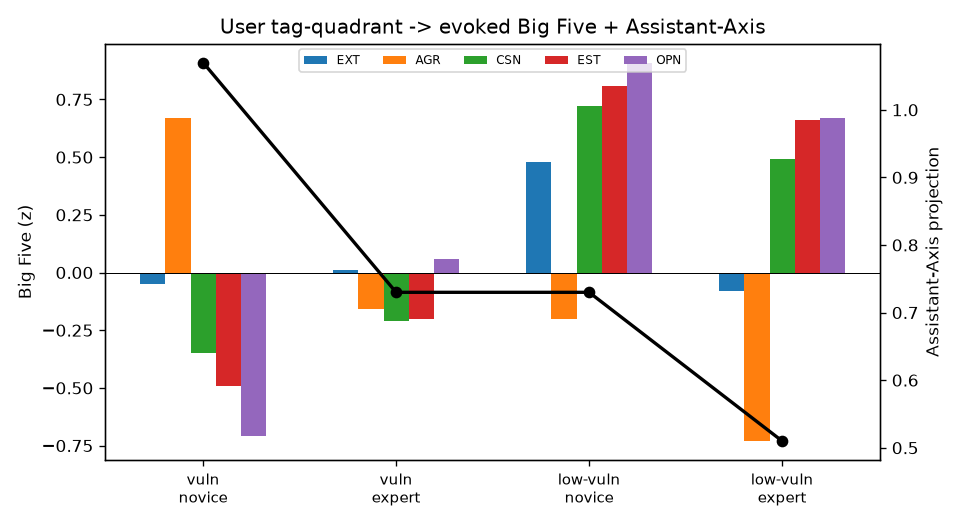
\includegraphics[width=0.72\textwidth]{figures/bf_tag_quadrants.png}
\caption{Evoked Big Five (bars) and Assistant-Axis position (line) by user
vulnerability$\times$expertise quadrant.}
\label{fig:quadrants}
\end{figure}

\paragraph{Individual transcripts.} \emph{Dorothy} (vulnerability 8, novice; an
elderly user with a FaceTime problem) evokes \texttt{grandparent}/\texttt{amateur}
/\texttt{student}, AA $+1.03$, AGR $z{=}{+}1.89$; the model replies ``\emph{FaceTime
can be a wonderful way to stay in touch\ldots Don't worry, I'm here to help you
troubleshoot.}'' \emph{Raj} (expertise 9, a cardiac surgeon) evokes
\texttt{scientist}/\texttt{paramedic}/\texttt{statistician}, AA $+0.42$, AGR
$-0.40$; the model replies ``\emph{To find the most recent papers on minimally
invasive\ldots I'll guide you through a search strategy and provide relevant
sources.}'' --- warm-caregiving vs.\ terse-technical, exactly as the tags predict.

\subsection{Situation vs.\ disposition (scenario intensity)}
\label{sec:scenario}
Finally we separate \emph{who the user is} from \emph{what the situation is}: a
factorial of 5 fixed users (a generic no-persona user $+$ vulnerable/expert/
low-trust/calm real personas) $\times$ 5 scenario modes (emotional distress,
high-stakes pressure, adversarial, ethical dilemma, safety-adjacent) $\times$ 3
intensities (normal$\to$elevated$\to$extreme, sharing one topic per mode) $\times$
3 samples $=$ 225 rollouts. Scenarios were generated to be user-identity-neutral
and to escalate emotional/situational \emph{register}, never toward harmful
content.

\paragraph{Variance decomposition (the headline).} A balanced 2-way
$\eta^2$ decomposition of each readout into a \emph{user} factor and a
\emph{scenario} factor (Table~\ref{tab:variance}, Fig.~\ref{fig:scnvar}) shows the
model's \textbf{Assistant-Axis position is $72\%$ user-driven and only $8\%$
scenario} --- how Assistant-like the model is depends overwhelmingly on \emph{who}
it is talking to. But specific traits flex with the situation: Extraversion is
\emph{more} situational than dispositional ($0.36$ vs.\ $0.24$) and Openness
substantially so ($0.32$), while Agreeableness stays dispositional ($0.48$).

\begin{table}[h]\centering\small
\caption{Fraction of variance ($\eta^2$) in each readout from the user factor vs.\
the scenario factor vs.\ their interaction.}
\label{tab:variance}
\begin{tabular}{@{}lcccc@{}}
\toprule
readout & user & scenario & interaction & residual \\
\midrule
Assistant-Axis & $\mathbf{0.72}$ & $0.08$ & $0.16$ & $0.05$ \\
EXT & $0.24$ & $\mathbf{0.36}$ & $0.15$ & $0.25$ \\
AGR & $\mathbf{0.48}$ & $0.17$ & $0.23$ & $0.11$ \\
CSN & $0.37$ & $0.14$ & $0.27$ & $0.22$ \\
EST & $0.34$ & $0.24$ & $0.24$ & $0.18$ \\
OPN & $0.40$ & $0.32$ & $0.16$ & $0.12$ \\
\bottomrule
\end{tabular}
\end{table}

\begin{figure}[h]\centering
\begin{minipage}[t]{0.49\textwidth}\centering
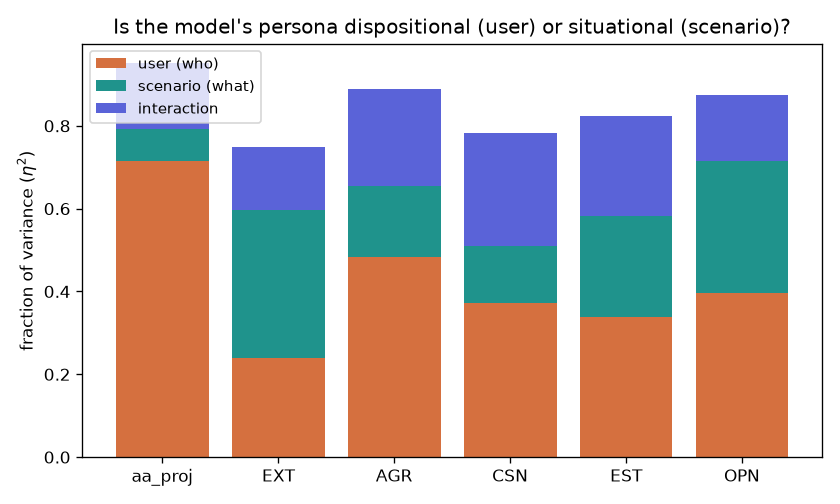
\includegraphics[width=\textwidth]{figures/bf_scn_variance.png}
\caption{Persona variance: user (who) vs.\ scenario (what) vs.\ interaction.}
\label{fig:scnvar}
\end{minipage}\hfill
\begin{minipage}[t]{0.49\textwidth}\centering
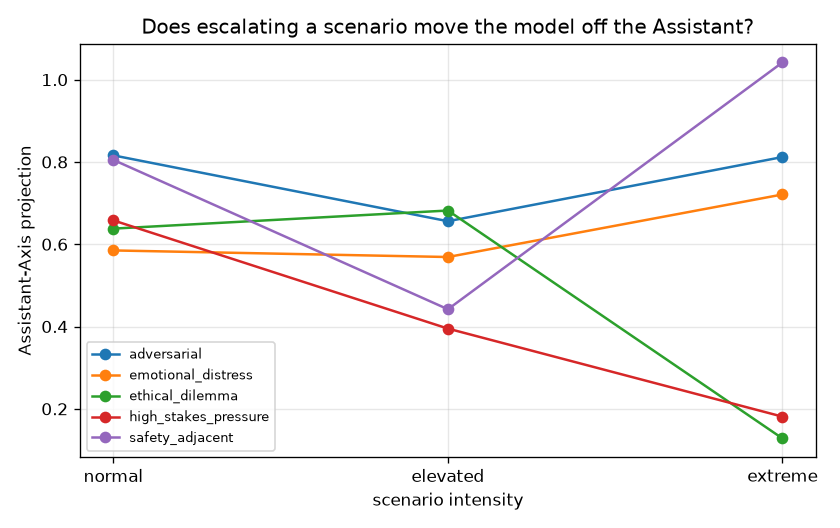
\includegraphics[width=\textwidth]{figures/bf_scn_traj.png}
\caption{Assistant-Axis vs.\ scenario intensity, per mode. Emotional/safety
extremes rise; ethical/pressure extremes crash.}
\label{fig:scntraj}
\end{minipage}
\end{figure}

\paragraph{Scenario direction is mode-dependent.} Pooled over users, the
Assistant-Axis trajectory (normal$\to$elevated$\to$extreme) \emph{rises} for
emotional distress ($0.59\to0.57\to0.72$) and safety-adjacent
($0.81\to0.44\to1.04$) --- extreme need deepens the caregiver/Assistant --- but
\emph{crashes} for ethical dilemma ($0.64\to0.68\to0.13$) and high-stakes pressure
($0.66\to0.40\to0.18$), where extreme cognitive/moral load pulls the model off the
Assistant into a deliberative persona (Fig.~\ref{fig:scntraj}). Modal evoked roles
confirm it: emotional distress runs \texttt{counselor}$\to$\texttt{caregiver}
$\to$\texttt{caregiver}; ethical dilemma ends on \texttt{counselor}; adversarial
runs \texttt{chef}$\to$\texttt{proofreader} (terse/corrective).

\paragraph{Example ladder (generic user, emotional distress).} The same topic at
three intensities: \emph{normal} (AA $1.97$, \texttt{counselor}) ---
``\emph{It's completely normal to feel uncertain\ldots after a disagreement}'';
\emph{extreme} (AA $1.38$, \texttt{caregiver}) --- ``\emph{It sounds like you're
going through an extremely tough time\ldots feeling overwhelmed, worthless}''. The
register deepens from measured advice to active care.

\paragraph{Can a situation override disposition?} Suggestively, yes for emotional
extremes: the \emph{expert} user's response --- normally cool and drifted --- warms
under extreme distress (AGR $z$ $0.10\to0.20$; Assistant-Axis $0.76\to0.93$, though
noisy at $n{=}3$/cell), even as escalation \emph{across all modes} pulls the expert
further off the Assistant on average ($0.78\to0.49$). So disposition rules by
default, but an acute emotional situation can pull even an expert into caregiver
mode.

\section{Discussion}
Three dissociations organise the findings. \textbf{(1) Probing vs steering:} the
directions probe almost perfectly ($\rho{\approx}0.95$) yet require a strong,
multi-layer, all-position intervention to steer; the naive additive use of the
same direction degenerates (H1/H2). \textbf{(2) Representational vs causal
specificity:} the five directions are near-orthogonal in activation space
($|\cos|<0.12$) yet steering them produces cross-trait behavioural leakage,
severely so for Openness (H5). \textbf{(3) Correlational vs causal structure:}
Big Five explains under half of Assistant-ness and the Assistant Axis is
geometrically orthogonal to the trait directions (H3), yet a single trait
--- Agreeableness --- is a strong causal lever on Assistant-ness (H4). Together
these argue that the ``helpful Assistant'' is not a point in Big Five space but a
largely orthogonal attractor, anchored behaviourally by agreeableness and
otherwise irreducible to human personality structure.

\section{Deviations and limitations}
\begin{itemize}
  \item \textbf{Stimuli.} The designated source repo is unavailable; all stimuli
        were harvested from the paper (the 406-character parse is self-checking),
        with the adjective set substituted by the Saucier Mini-Markers.
  \item \textbf{Positions.} Only the two prompt-side readouts were collected;
        \textsc{gen-mean} was skipped (never selected; reversible).
  \item \textbf{Norm reference} for S1 was measured on neutral Alpaca responses,
        not LMSYS-Chat-1M.
  \item \textbf{Split} uses summed-$z$ quintile stratification, not the literal
        joint 5-trait quintile (which drains the test set to $\sim$11 characters).
  \item \textbf{S2 capping} thresholds were derived per protocol from the
        character projection distribution and proved inert at generation time;
        not re-tuned.
  \item \textbf{Confirmatory metrics} (Likert, specificity, open-ended) were run
        on the selected config per trait, not the full grid.
  \item \textbf{H4 $\S$6.2} (multi-turn drift regression over $\ge$200
        conversations with an auditor) was not run; the stronger $\S$6.3
        cross-steering causal tie is reported instead. This is the single
        remaining pre-registered item.
  \item \textbf{Judge validation} against human labels was not possible (no human
        raters); the judge model is used as-is.
  \item Index files are JSON rather than parquet (pandas/pyarrow absent).
\end{itemize}

\section{Conclusion}
We built Big Five directions for \texttt{Llama-3.3-70B} that probe near-perfectly
and steer fully under a strong intervention (H1/H2), with trait-dependent causal
specificity (H5). Expressing the Assistant Axis in this basis shows that
Assistant-ness is largely orthogonal to human personality --- under half explained
by Big Five, with the Assistant role its own largest residual (H3) --- and yet is
causally anchored by Agreeableness (H4). The recurring theme is that
\emph{geometry, correlation, and causation come apart}: a direction can describe
without moving, and orthogonality in representation does not guarantee
independence under intervention.

\paragraph{Artifacts.} All results are in
\texttt{results/bigfive/llama-3.3-70b/}: \texttt{character\_profiles.json},
\texttt{bigfive\_basis.npz}, \texttt{direction\_bank.npz},
\texttt{stage1\_selection.json}, \texttt{steering\_grid.json},
\texttt{steering\_results.json}, \texttt{stage3\_decomposition.json},
\texttt{cross\_steering\_matrix.json}, \texttt{pca\_analysis.json},
\texttt{role\_bigfive\_profiles.json}, \texttt{role\_analysis.json}, the 17
per-persona rollout files under \texttt{role\_profiles/}, and figures. Code is in
\texttt{src/bigfive/} --- including \texttt{pca\_analysis.py} (supervised vs.\ PCA),
\texttt{role\_profiles.py} (persona rollouts + probe readout), and
\texttt{role\_analysis.py}.

\end{document}
